\section{Measured Surface Temperatures}
\label{sec:res-thermal}

Heating became more pronounced as load increased in the \SI{9}{\volt}
and \SI{20}{\volt} image groups. The image labeled \SI{20}{\volt},
\SI{4}{\ampere} shows a \SI{90.4}{\celsius} maximum. At the labeled
\SI{20}{\volt}, \SI{4.7}{\ampere} condition, the maximum is
\SI{102.9}{\celsius}, the highest recorded surface reading.

\begin{figure}[htbp]
\centering
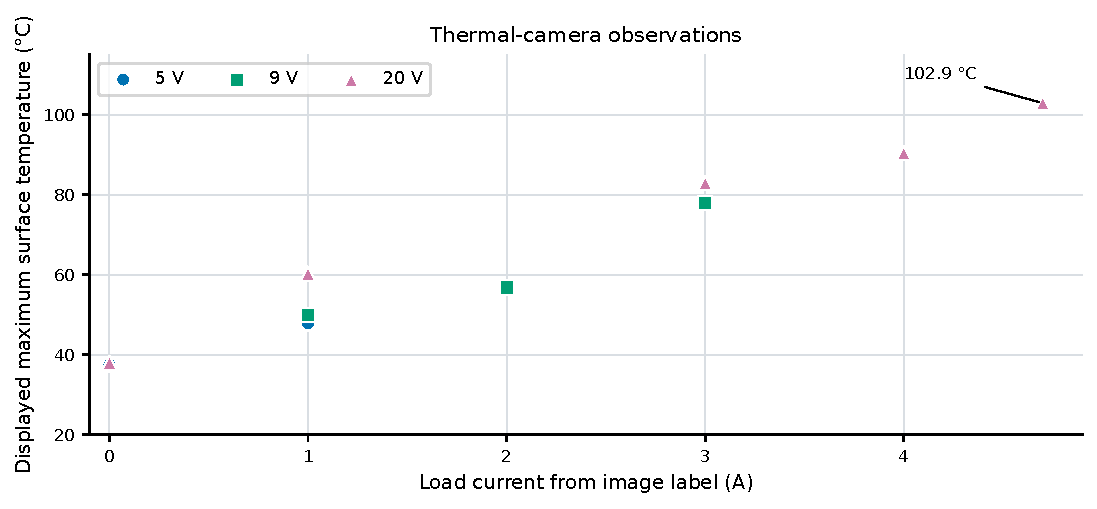
\includegraphics[width=0.95\textwidth]{Pictures/Thesis/10_Results/Rebuilt/thermal_observations.pdf}
\caption{Maximum surface temperatures in the ten thermal images, using the load conditions written on each image. Run duration and airflow were not recorded, so thermal equilibrium cannot be checked.}
\label{fig:rebuilt-thermal}
\end{figure}

The ten no-load and loaded images use an emissivity of 0.95. At
\SI{9}{\volt} and \SI{2}{\ampere}, the camera maximum was
\SI{56.8}{\celsius}, while the cursor read
\SI{39.7}{\celsius}. The plotted temperatures are camera maxima.

\begin{figure}[htbp]
\centering
\begin{subfigure}[t]{0.31\textwidth}
\centering
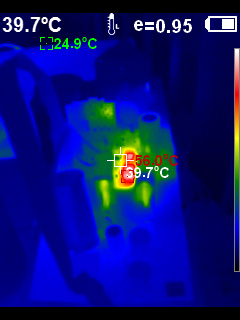
\includegraphics[width=\linewidth,height=0.27\textheight,keepaspectratio]{Pictures/Thesis/10_Results/image_009_9v_2a.png}
\caption{\SI{9}{\volt}, \SI{2}{\ampere}.}
\end{subfigure}\hfill
\begin{subfigure}[t]{0.31\textwidth}
\centering
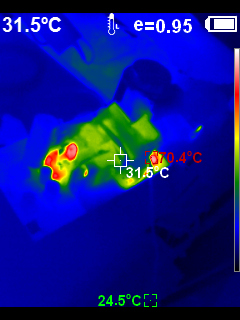
\includegraphics[width=\linewidth,height=0.27\textheight,keepaspectratio]{Pictures/Thesis/10_Results/image_006_20v_4a.png}
\caption{\SI{20}{\volt}, \SI{4}{\ampere}.}
\end{subfigure}\hfill
\begin{subfigure}[t]{0.31\textwidth}
\centering
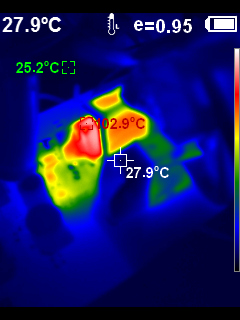
\includegraphics[width=\linewidth,height=0.27\textheight,keepaspectratio]{Pictures/Thesis/10_Results/image_001_20v_4p7a.png}
\caption{\SI{20}{\volt}, \SI{4.7}{\ampere}.}
\end{subfigure}
\caption{Thermal images with their camera readings and test labels.}
\label{fig:thermal-9v-2a-hotspot}
\end{figure}

% Automatically rebuilt from original records by rebuild_results.py.
\begingroup
\scriptsize
\setlength{\tabcolsep}{3pt}
\renewcommand{\arraystretch}{1.12}
\begin{longtable}{@{}L{0.3400\linewidth} L{0.1800\linewidth} L{0.1800\linewidth} L{0.1800\linewidth}@{}}
\caption{Temperature readings from ten thermal images, using emissivity 0.95. The lower reference marker was not confirmed as ambient temperature.}\label{tab:thermal-results}\\
\toprule
Image / condition & Maximum (°C) & Cursor (°C) & Reference (°C)\\
\midrule
\endfirsthead
\toprule
Image / condition & Maximum (°C) & Cursor (°C) & Reference (°C)\\
\midrule
\endhead
Image \#1 / 20 V, 4.7 A & 102.9 & 27.9 & 25.2\\
Image \#2 / 20 V, 1 A & 60.3 & 30.8 & 24.9\\
Image \#3 / 20 V, 3 A & 82.9 & 30.6 & 25.2\\
Image \#4 / 5 V, 1 A & 47.8 & 29.1 & 24.7\\
Image \#5 / 20 V, no load & 38.0 & 29.2 & 25.4\\
Image \#6 / 20 V, 4 A & 90.4 & 31.5 & 24.5\\
Image \#7 / 5 V, open & 37.5 & 34.9 & 25.5\\
Image \#8 / 9 V, 1 A & 49.9 & 29.6 & 25.0\\
Image \#9 / 9 V, 2 A & 56.8 & 39.7 & 24.9\\
Image \#10 / 9 V, 3 A & 78.0 & 32.1 & 25.3\\
\bottomrule
\end{longtable}
\endgroup


Hotspot components are incompletely identified, junction temperatures were
not measured, and lower reference markers are not ambient readings. Missing
duration, airflow, camera distance, and temperature histories prevent a
steady-state thermal comparison. The \SI{4.7}{\ampere} record also lacks DC output
voltage, so output power for the nominal \SI{94}{\watt} point cannot be calculated.

The matched electrical results reach approximately \SIrange{74}{80}{\watt}.
Continuous capability requires a stabilized run with identified hotspots,
controlled ambient/airflow, and device and insulation acceptance limits.
